\documentclass[12pt,letterpaper]{article}
\usepackage[utf8]{vietnam}
\usepackage{fullpage}
\usepackage[top=2cm, bottom=4.5cm, left=2.5cm, right=2.5cm]{geometry}
\usepackage{amsmath,amsthm,amsfonts,amssymb,amscd}
\usepackage{lastpage}
\usepackage{enumerate}
\usepackage{fancyhdr}
\usepackage{mathrsfs}
\usepackage{xcolor}
\usepackage{graphicx}
\usepackage{listings}
\usepackage{hyperref}

\usepackage{caption}
\usepackage{subcaption}
\hypersetup{%
  colorlinks=true,
  linkcolor=blue,
  linkbordercolor={0 0 1}
}

\renewcommand\lstlistingname{Algorithm}
\renewcommand\lstlistlistingname{Algorithms}
\def\lstlistingautorefname{Alg.}

\lstdefinestyle{Python}{
    language        = Python,
    frame           = lines, 
    basicstyle      = \footnotesize,
    keywordstyle    = \color{blue},
    stringstyle     = \color{green},
    commentstyle    = \color{red}\ttfamily
}

\setlength{\parindent}{0.0in}
\setlength{\parskip}{0.05in}

% Edit these as appropriate
\newcommand\course{Massp2019}
\newcommand\hwnumber{MPB Report}                  % <-- homework number
\newcommand\NetIDa{Nguyen Quang Huy}           % <-- NetID of person #1

\pagestyle{fancyplain}
\headheight 35pt
\lhead{\NetIDa}
%\lhead{\NetIDa\\\NetIDb}                 % <-- Comment this line out for problem sets (make sure you are person #1)
\chead{\textbf{\Large Hw \hwnumber}}
\rhead{\course \\ \today}
\lfoot{}
\cfoot{}
\rfoot{\small\thepage}
\headsep 1.5em

\begin{document}
\section*{Multi-layer Perceptron là gì}
Multi-layer Perceptron sử dụng nhiều layer để tính toán thay vì chỉ dùng 1 layer như thuật toán Logistic Regression.
Các activation function là các hàm phi tuyến

Công thức của Multi-layer Perceptron là 
$$
    y =  \theta_n(w_n^T*(...\theta_2(w_2^T*\theta_1(w_1^T*x))
$$
\section*{Áp dụng vào bài toán}
Bài toán classification điểm dữ liệu:
\\
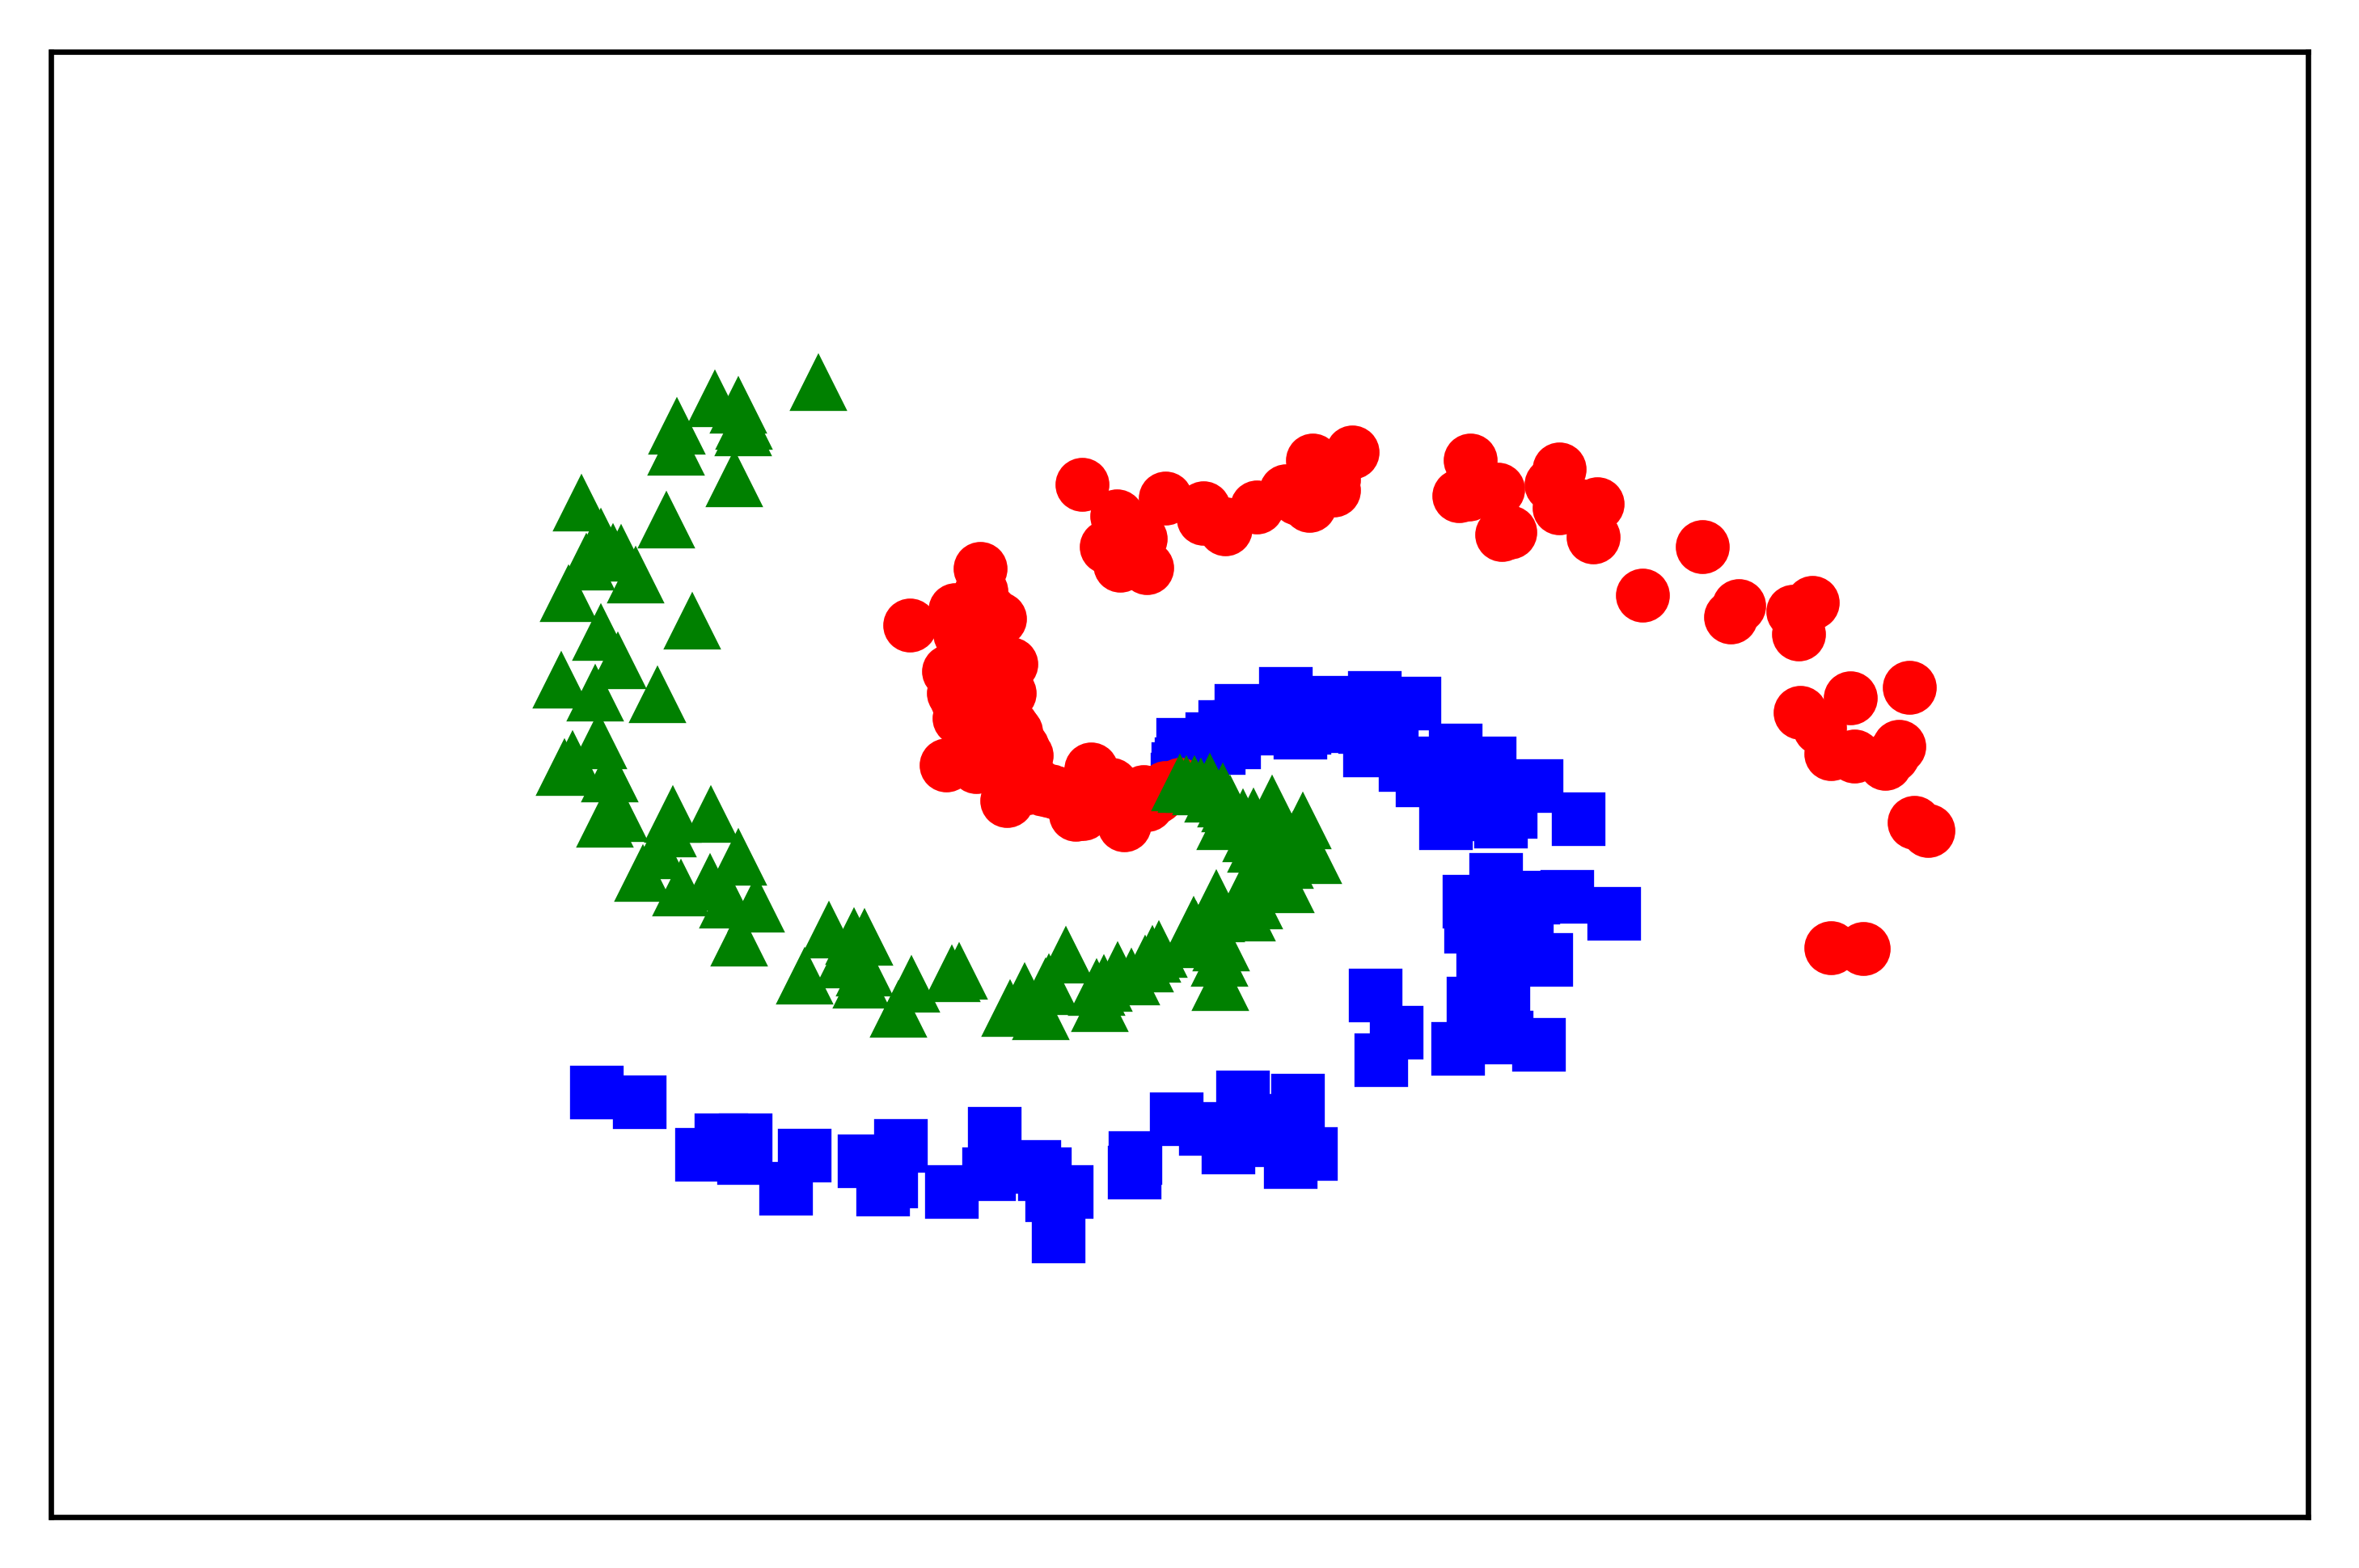
\includegraphics[width=1 \linewidth]{EX.png}

Nhận xét: loss function giảm khi tăng số lượng hidden layer\\
Với số lượng hàm ẩn lần lượt là 10,20,50,100,200,500 ta có:

\begin{figure}
\captionsetup[subfigure]{labelformat=empty}
\centering
\begin{subfigure}{.5\textwidth}
  \centering
  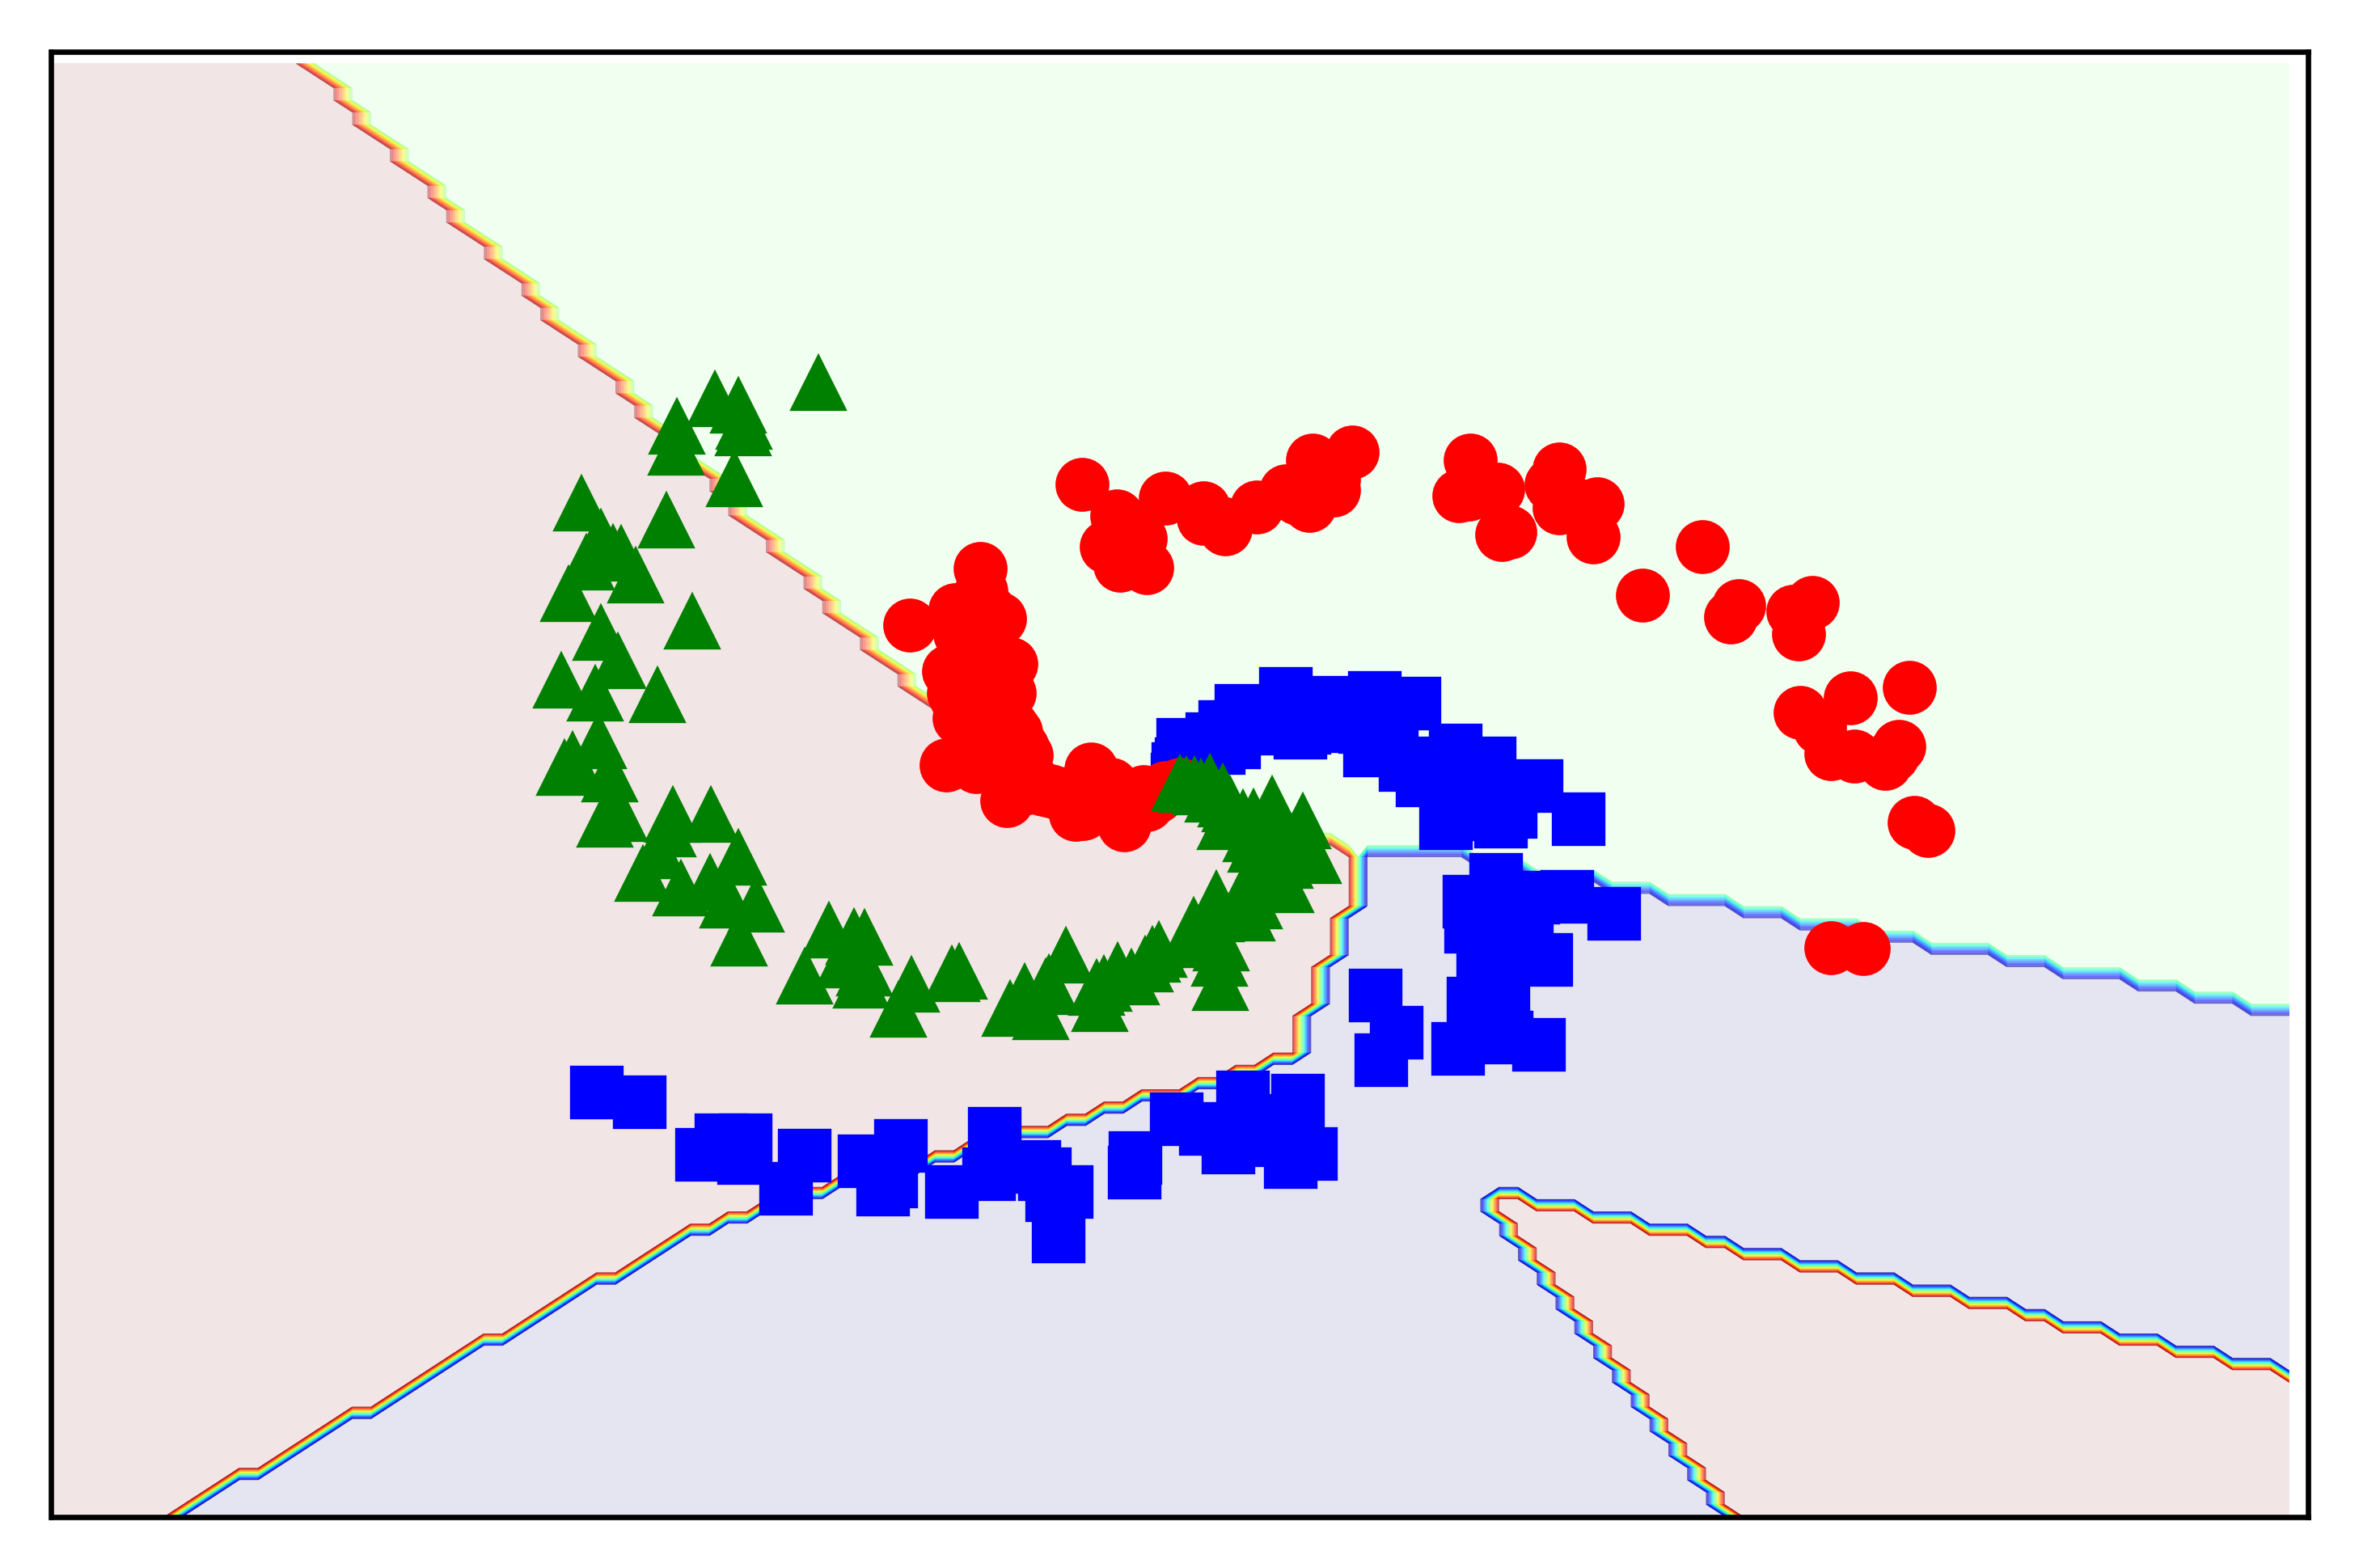
\includegraphics[width=1\linewidth]{EX10.png}
  \caption{K = 10}
  \label{fig:sub1}
\end{subfigure}%
\begin{subfigure}{.5\textwidth}
  \centering
  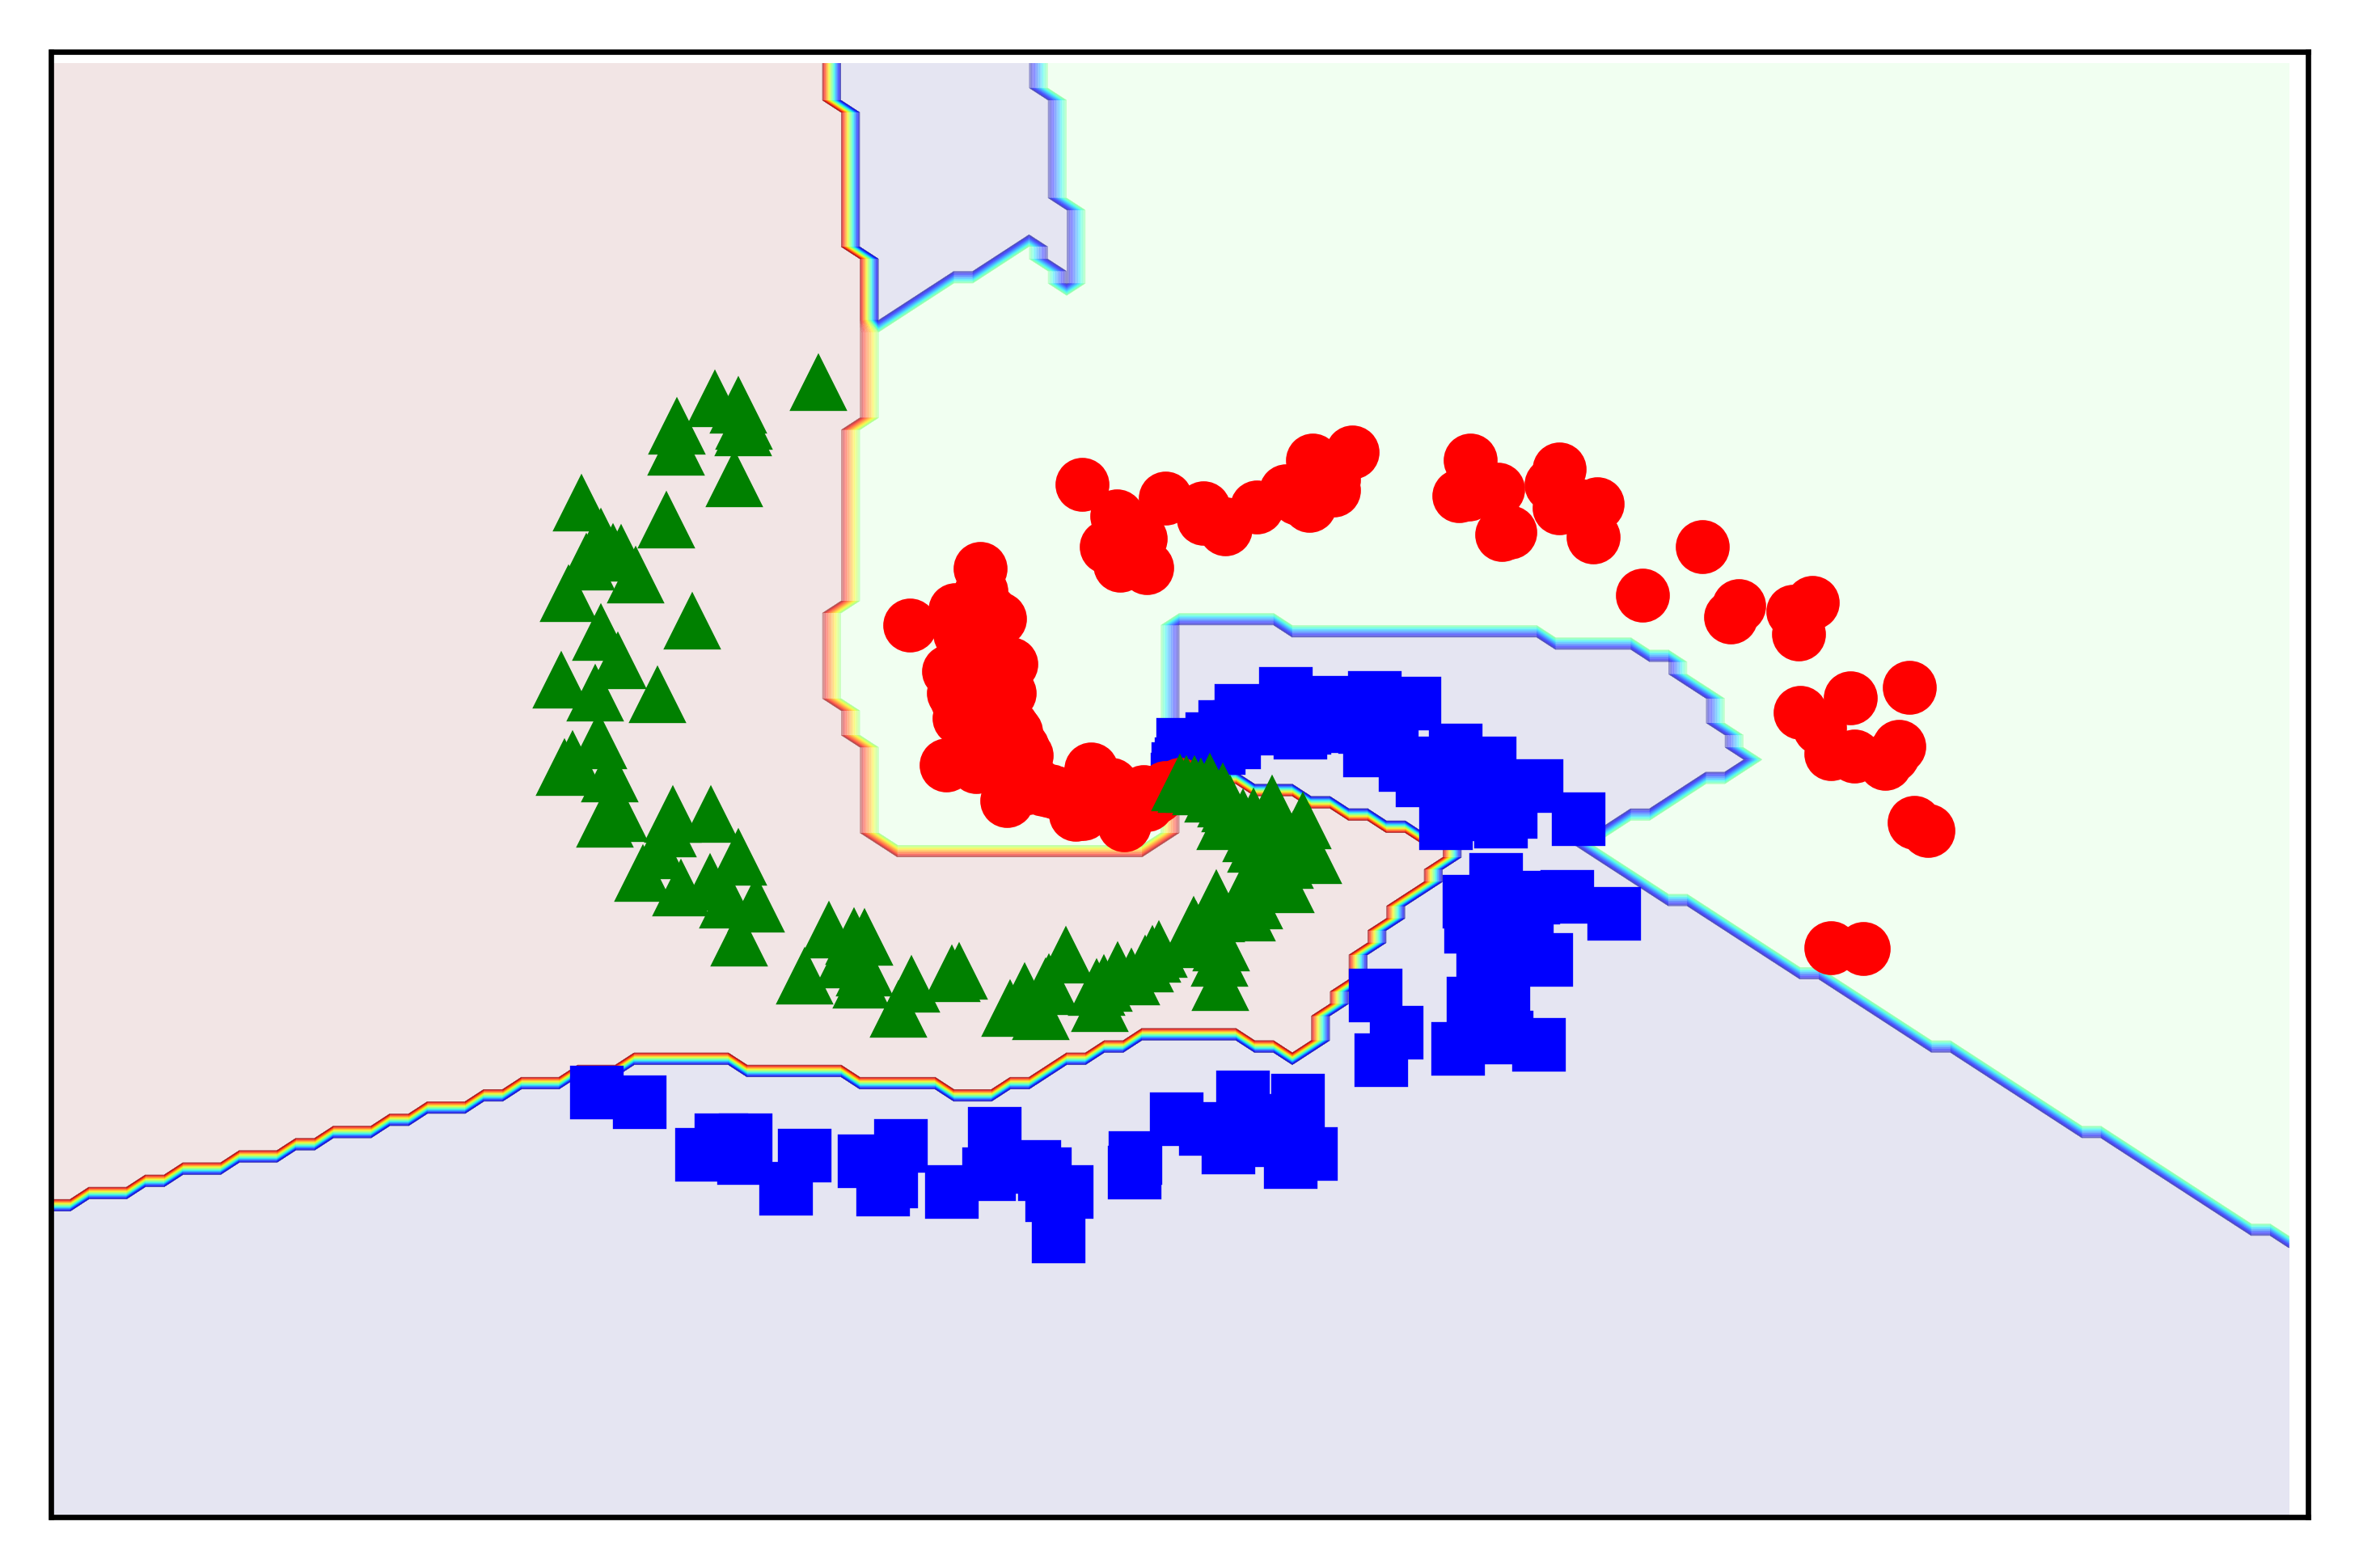
\includegraphics[width=1\linewidth]{EX20.png}
  \caption{K = 20}
  \label{fig:sub2}
\end{subfigure}
\label{fig:test}
\end{figure}


\begin{figure}
\captionsetup[subfigure]{labelformat=empty}
\centering
\begin{subfigure}{.5\textwidth}
  \centering
  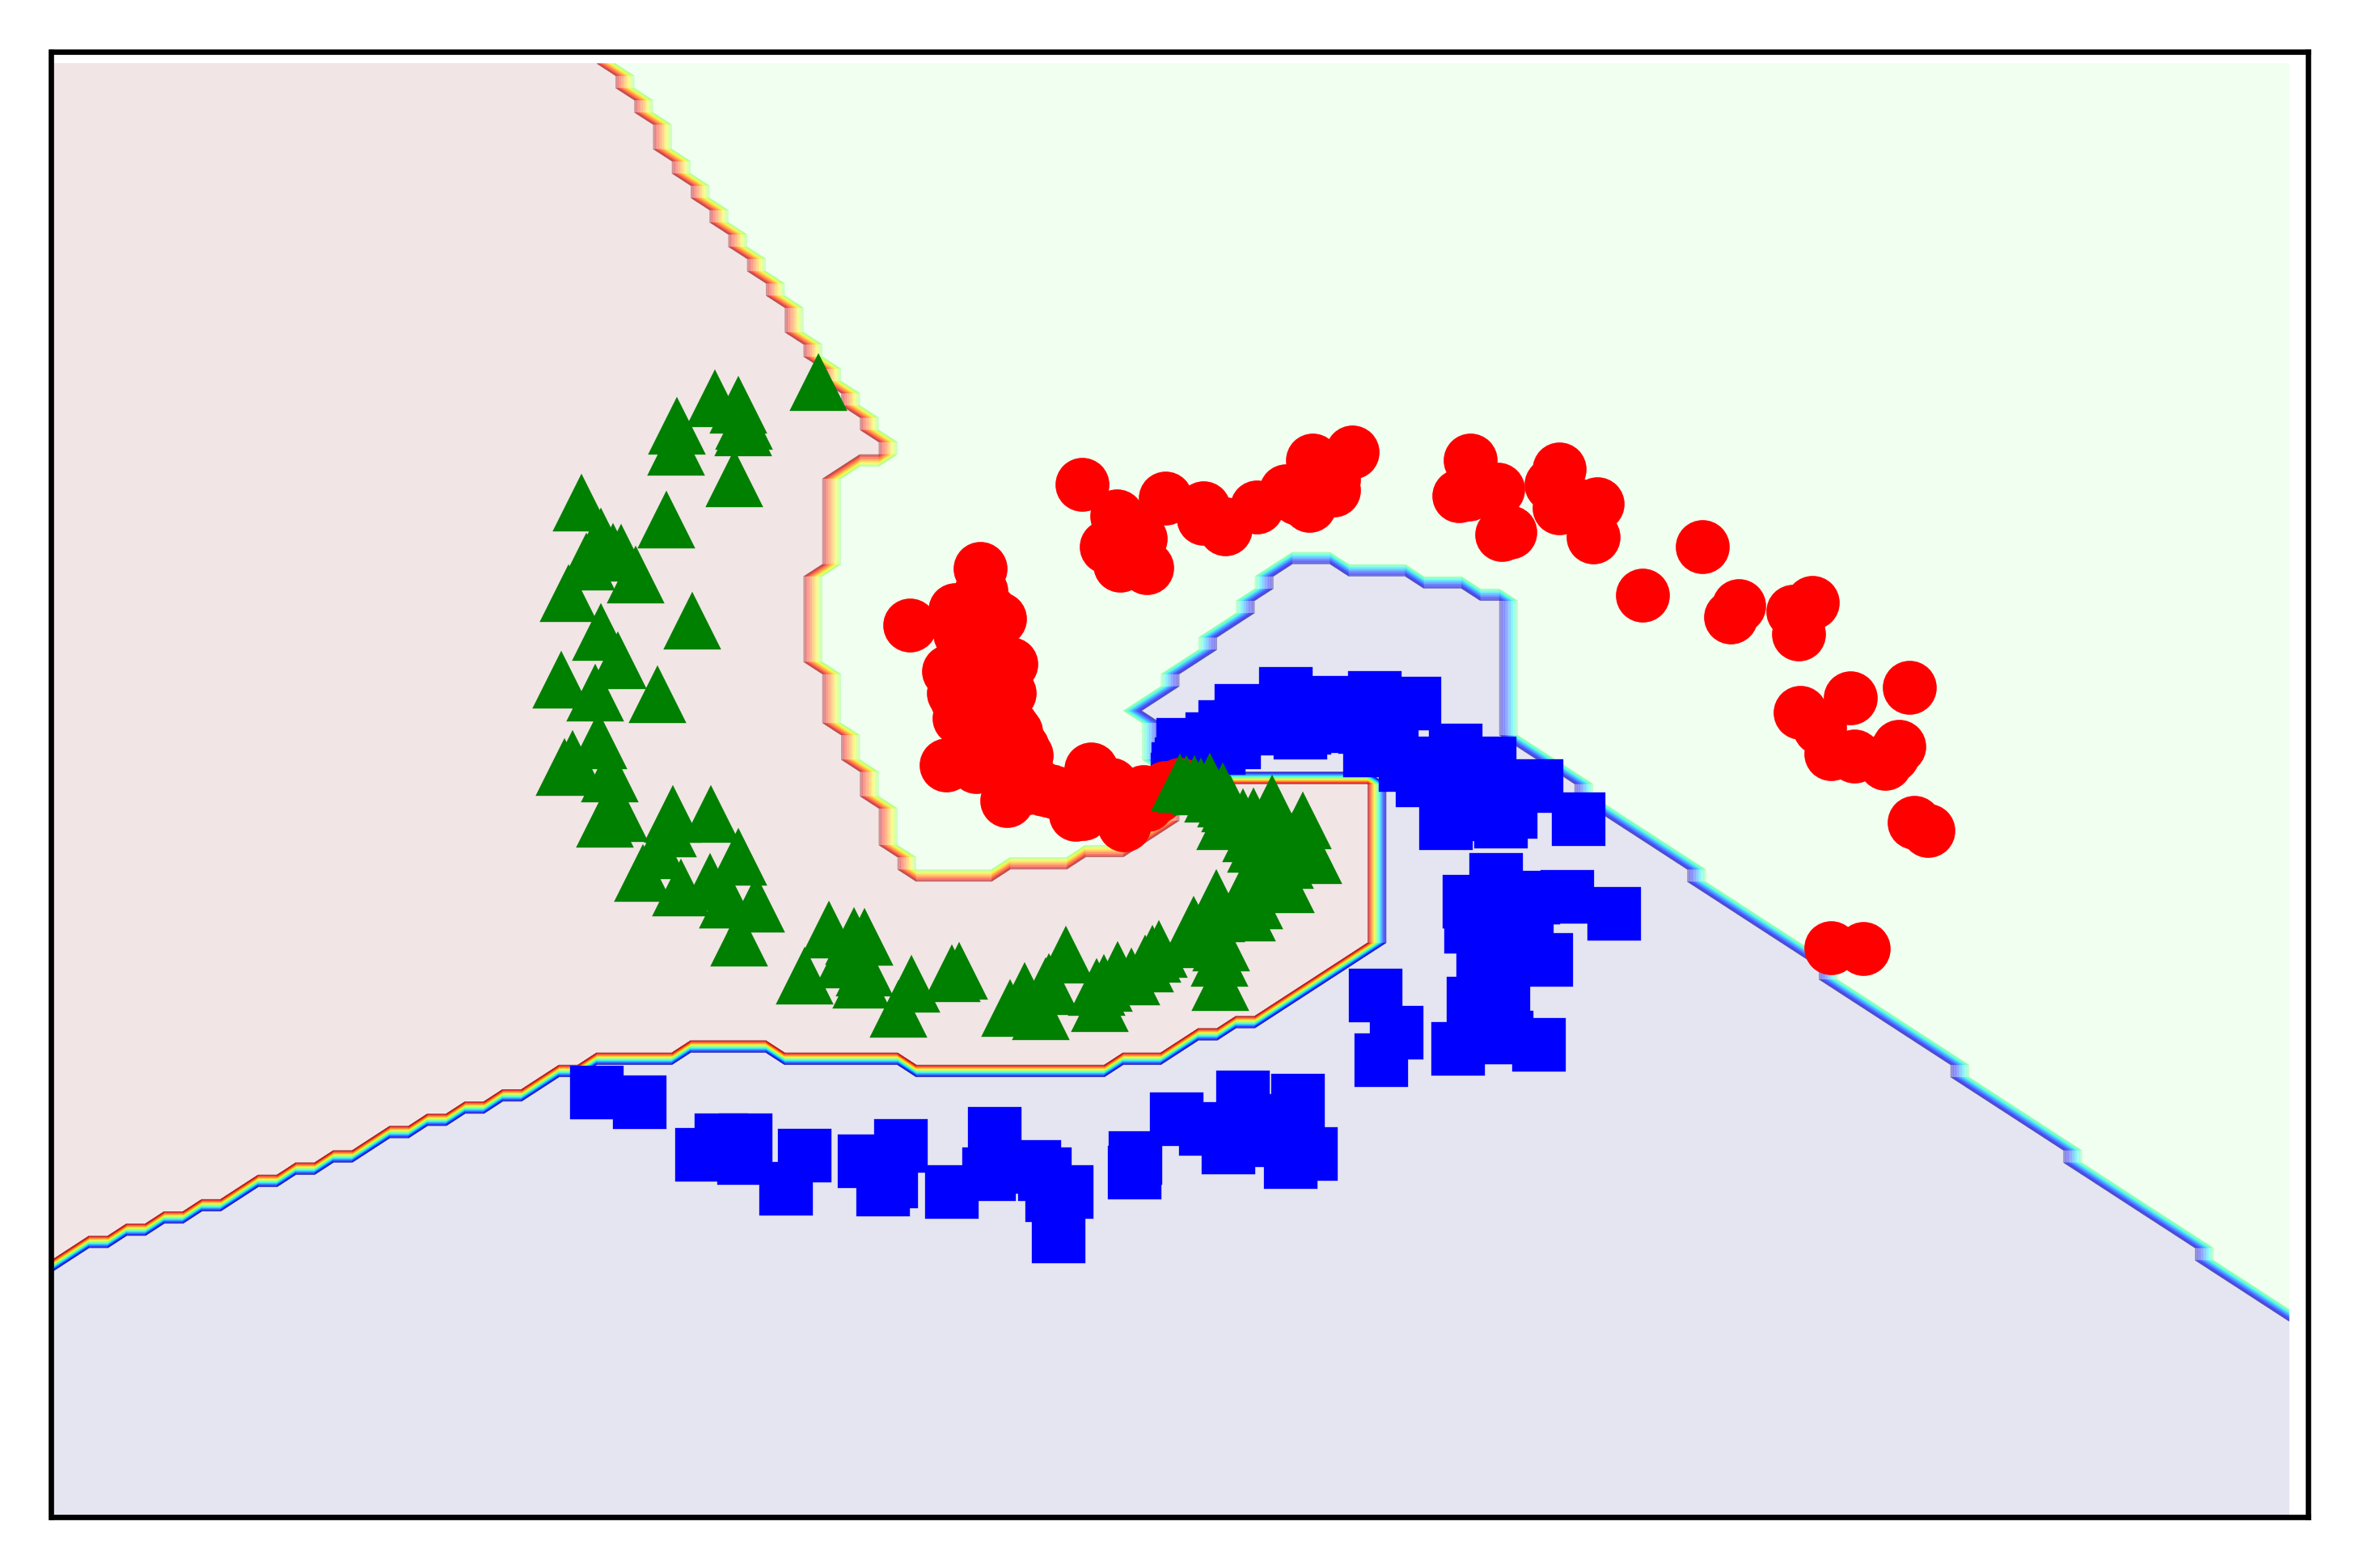
\includegraphics[width=1\linewidth]{EX50.png}
  \caption{K = 50}
  \label{fig:sub1}
\end{subfigure}%
\begin{subfigure}{.5\textwidth}
  \centering
  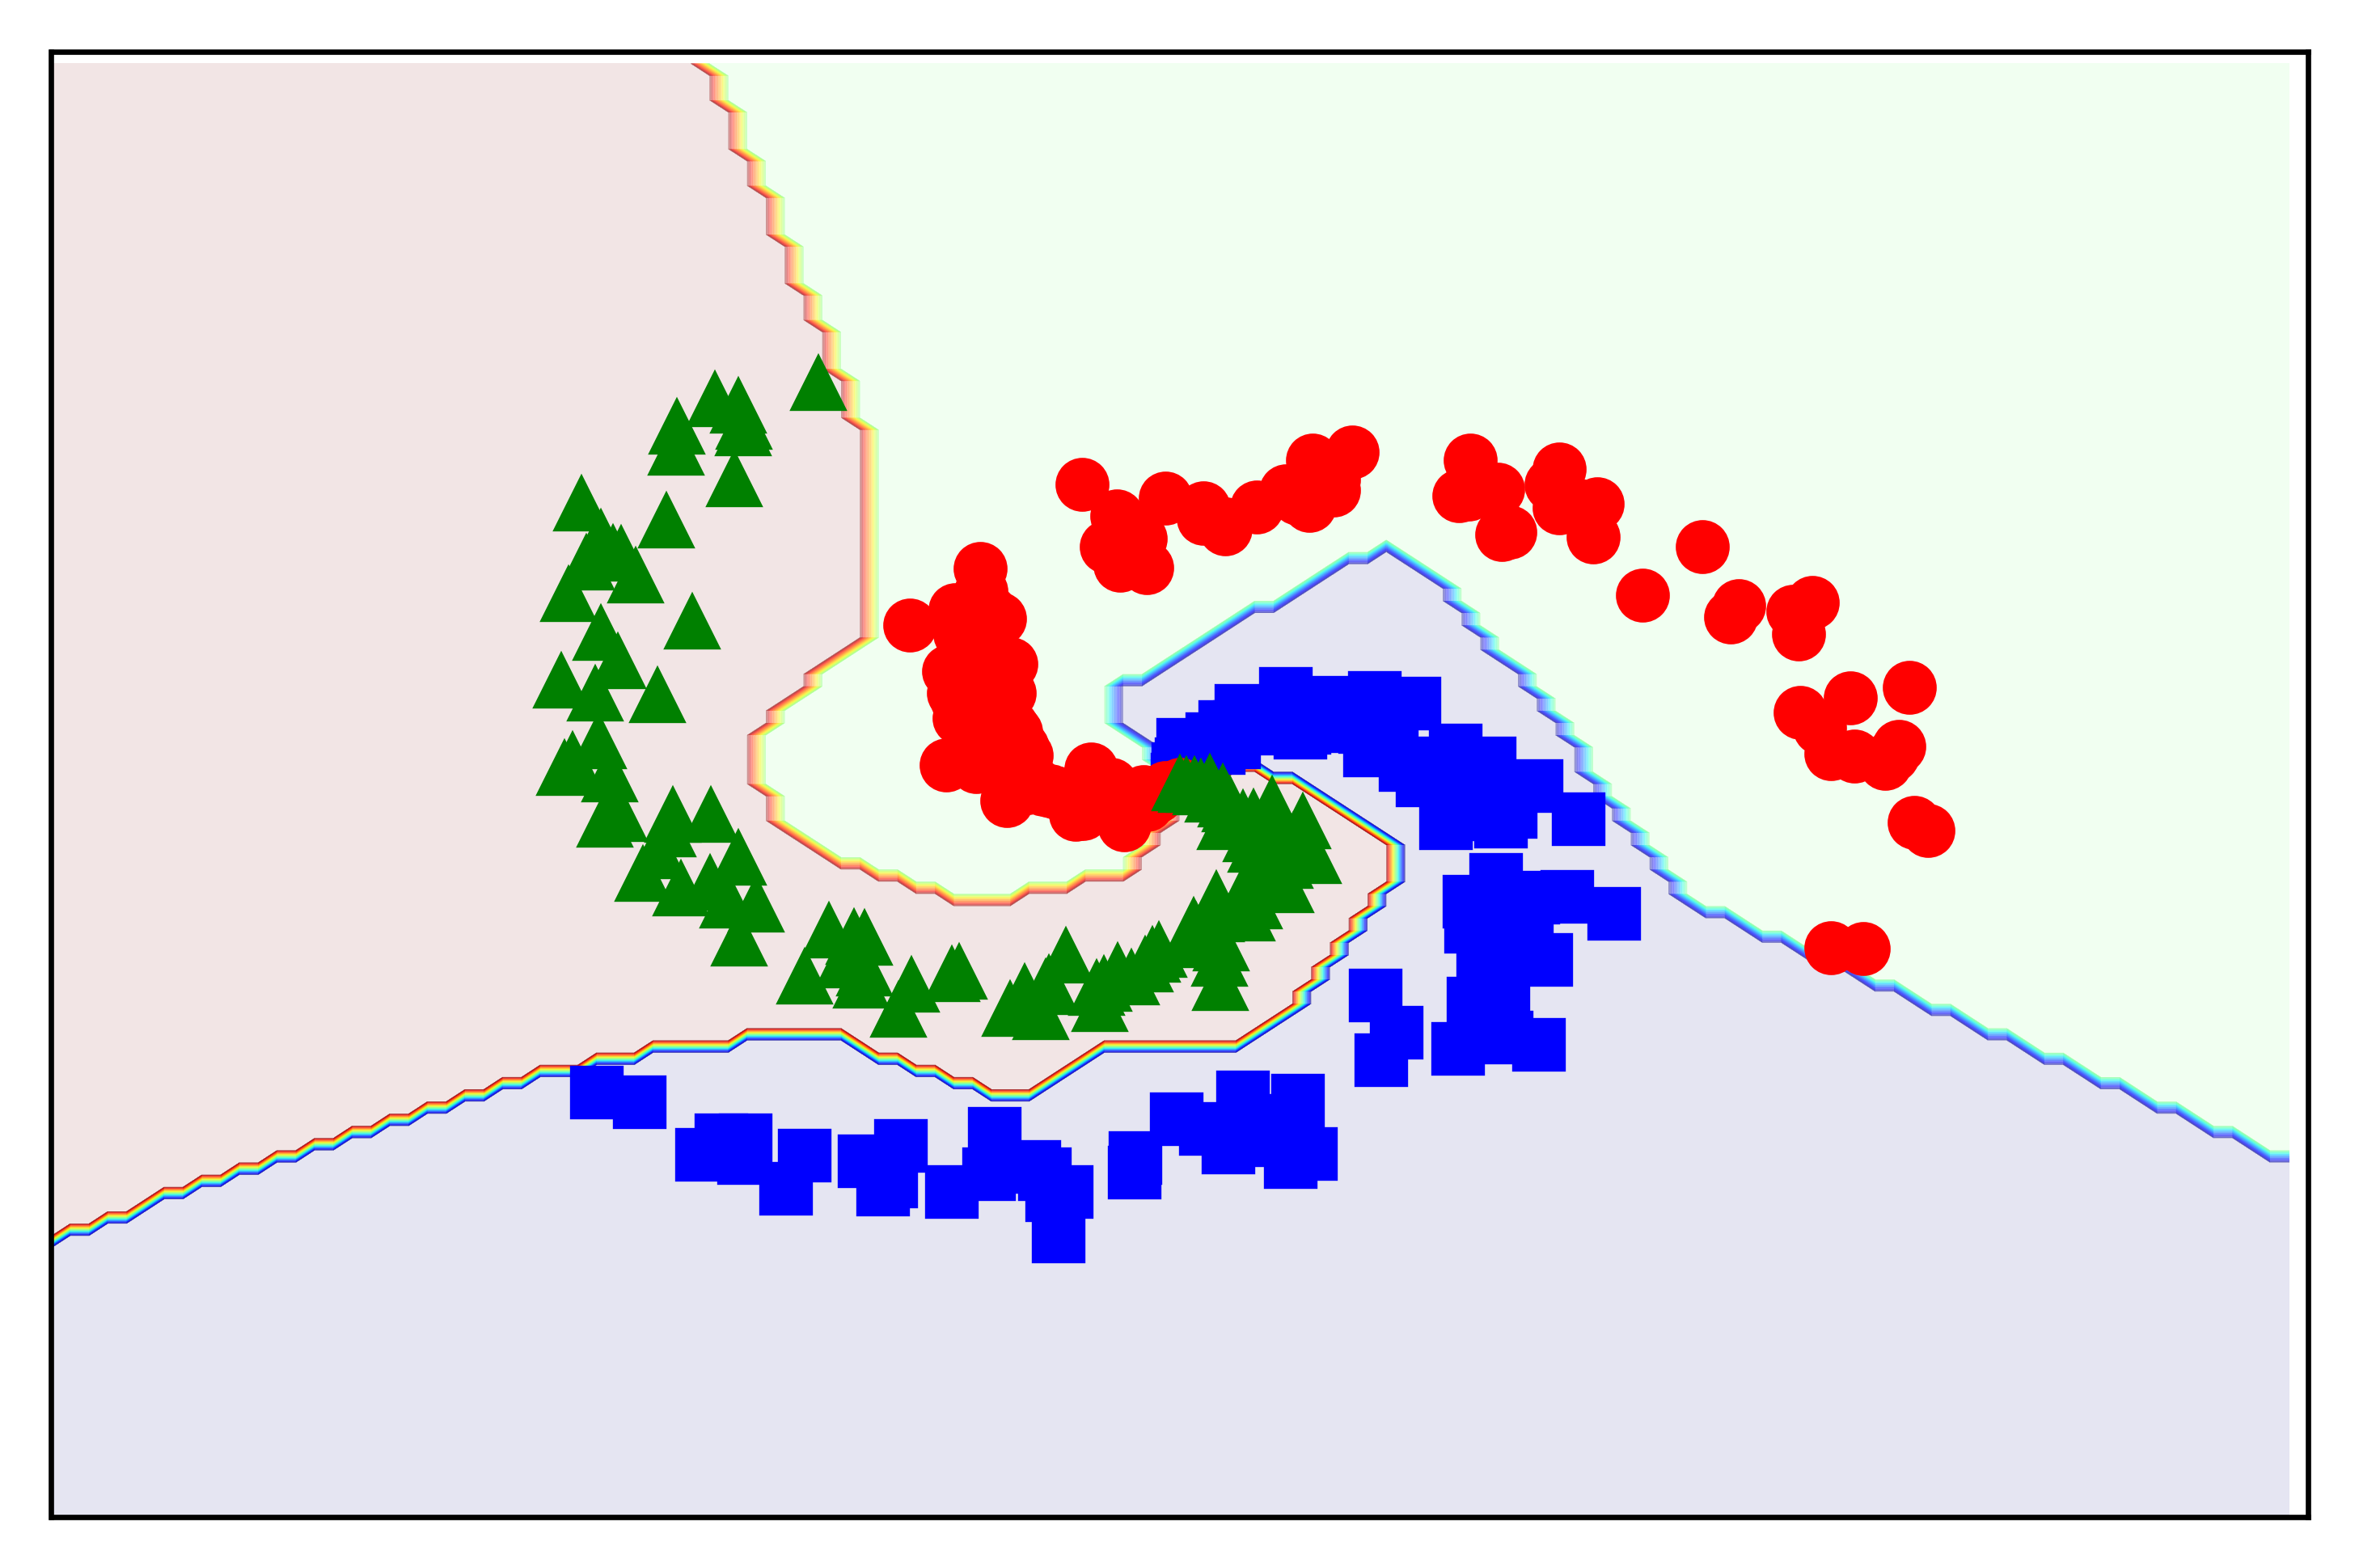
\includegraphics[width=1\linewidth]{EX100.png}
  \caption{K = 100}
  \label{fig:sub2}
\end{subfigure}
\label{fig:test}
\end{figure}


\begin{figure}
\captionsetup[subfigure]{labelformat=empty}
\centering
\begin{subfigure}{.5\textwidth}
  \centering
  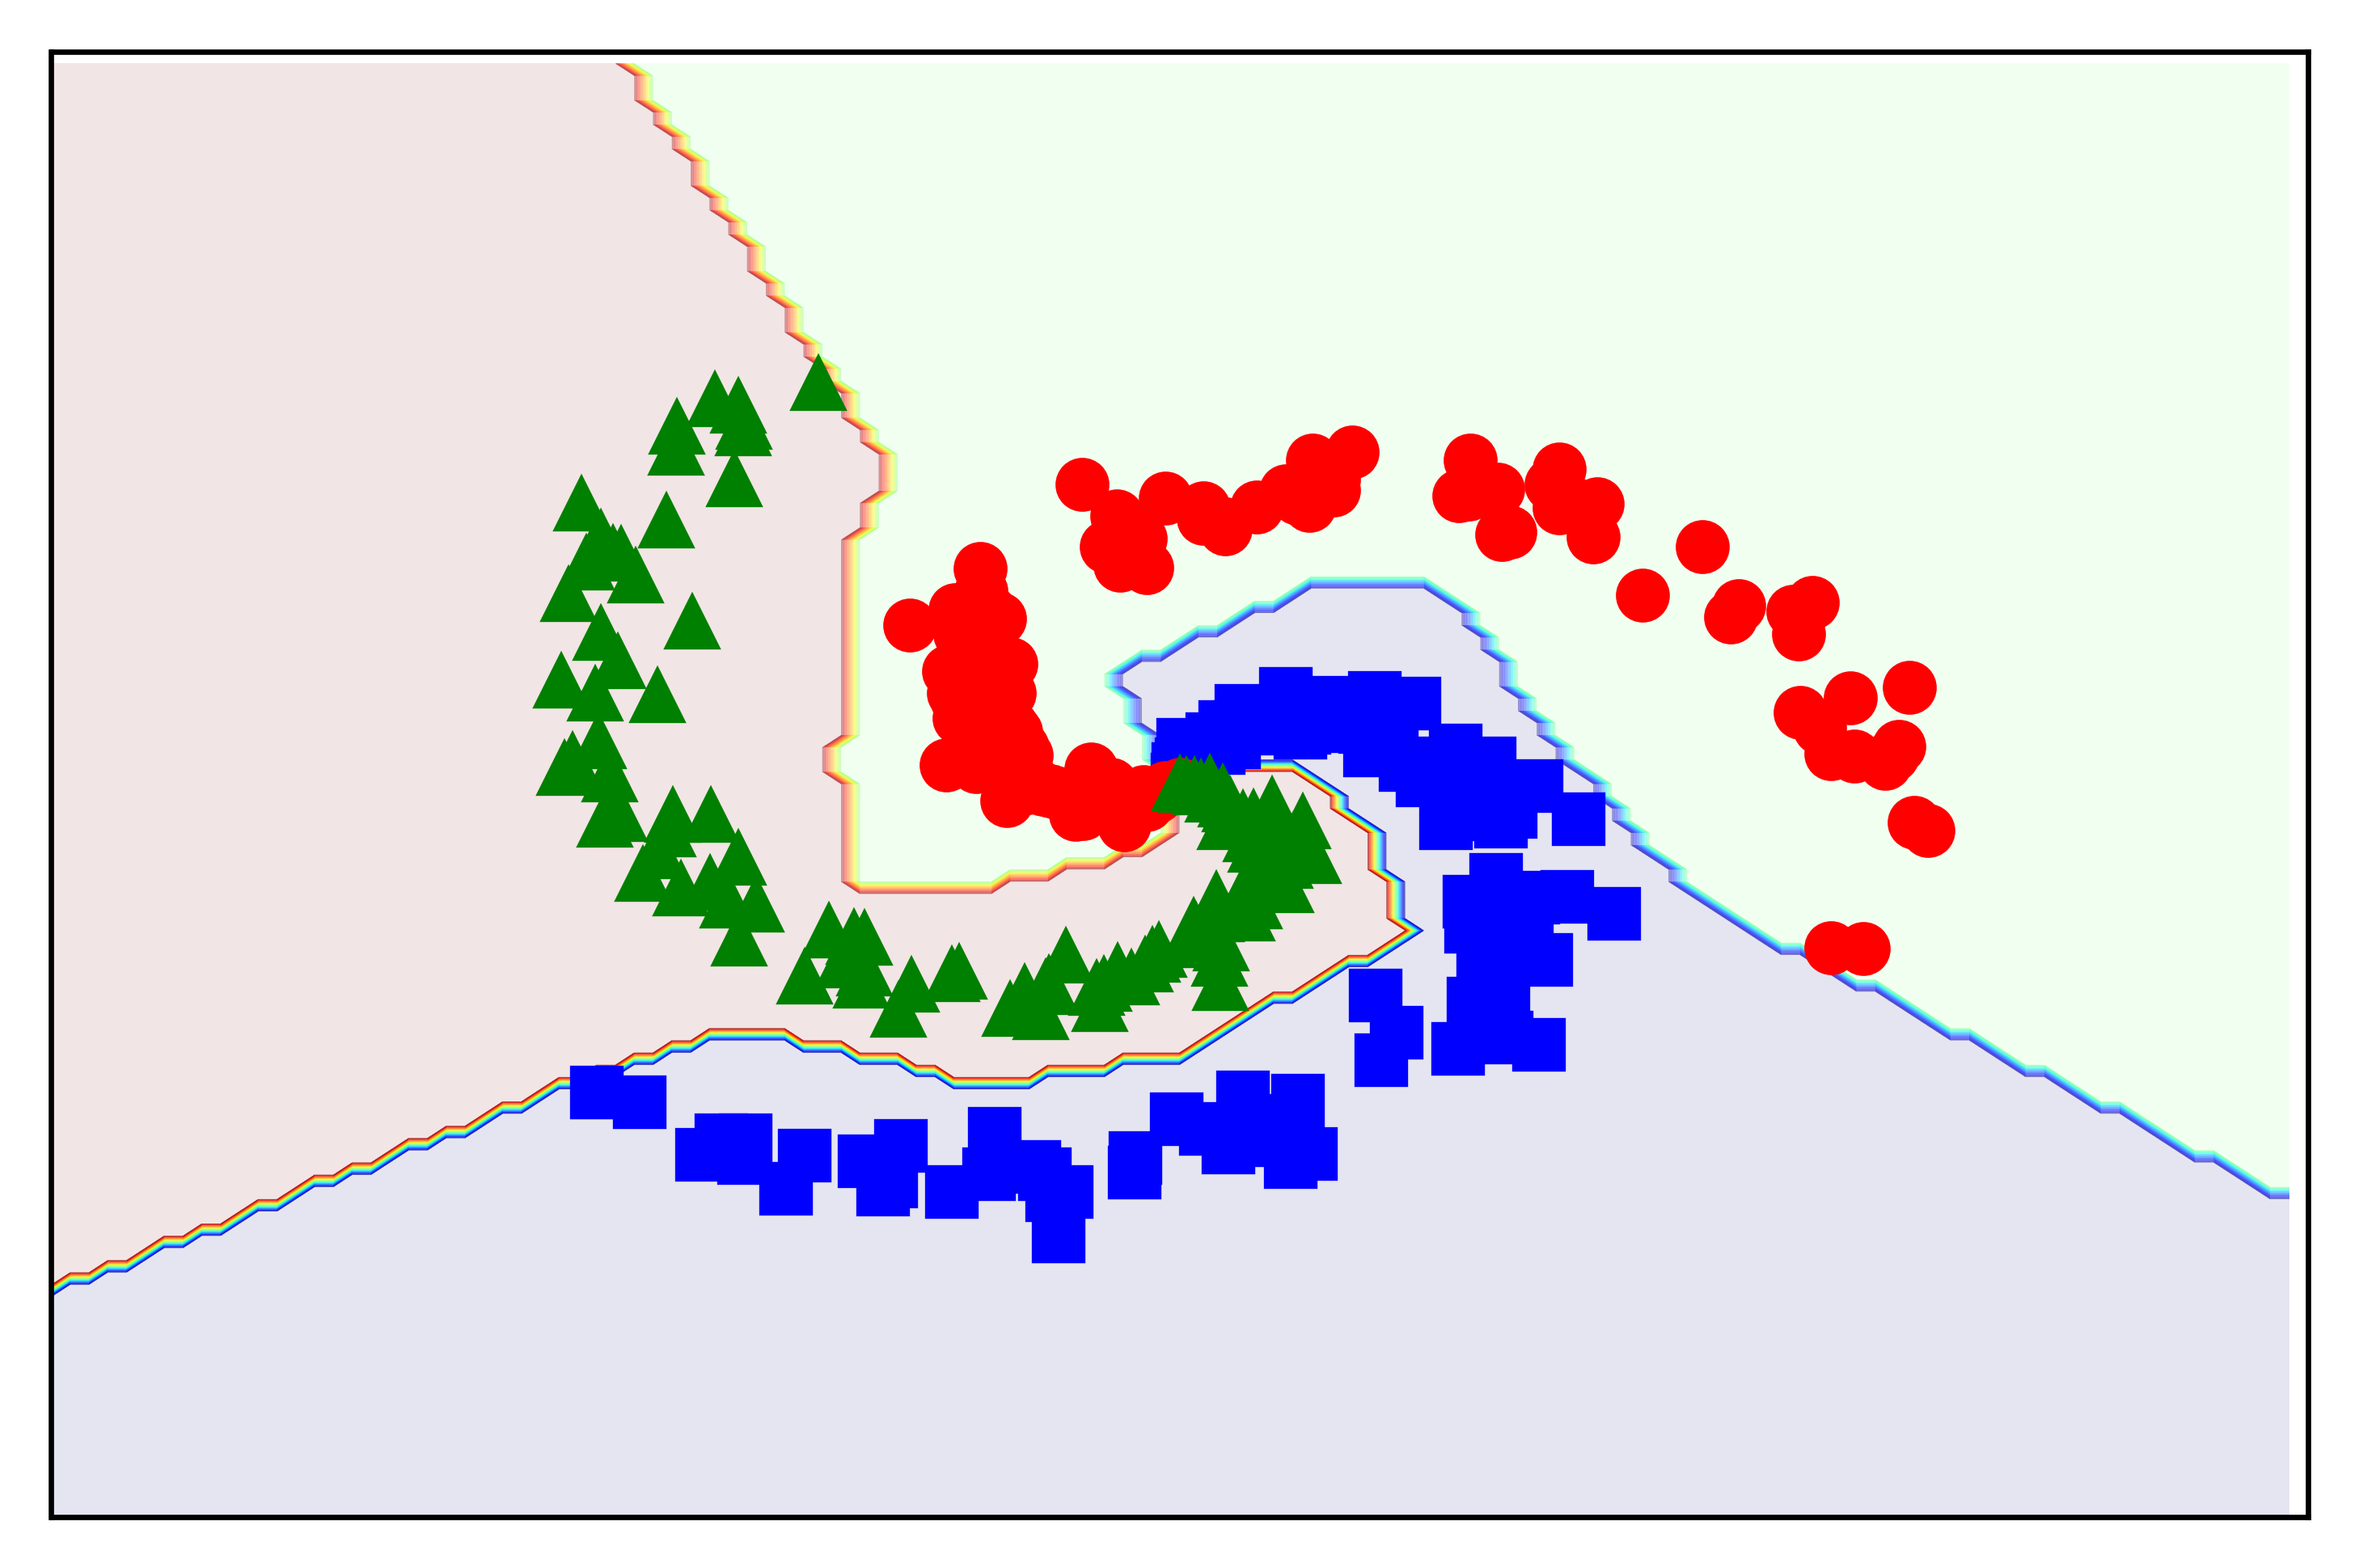
\includegraphics[width=1\linewidth]{EX200.png}
  \caption{K = 200}
  \label{fig:sub3}
\end{subfigure}%
\begin{subfigure}{.5\textwidth}
  \centering
  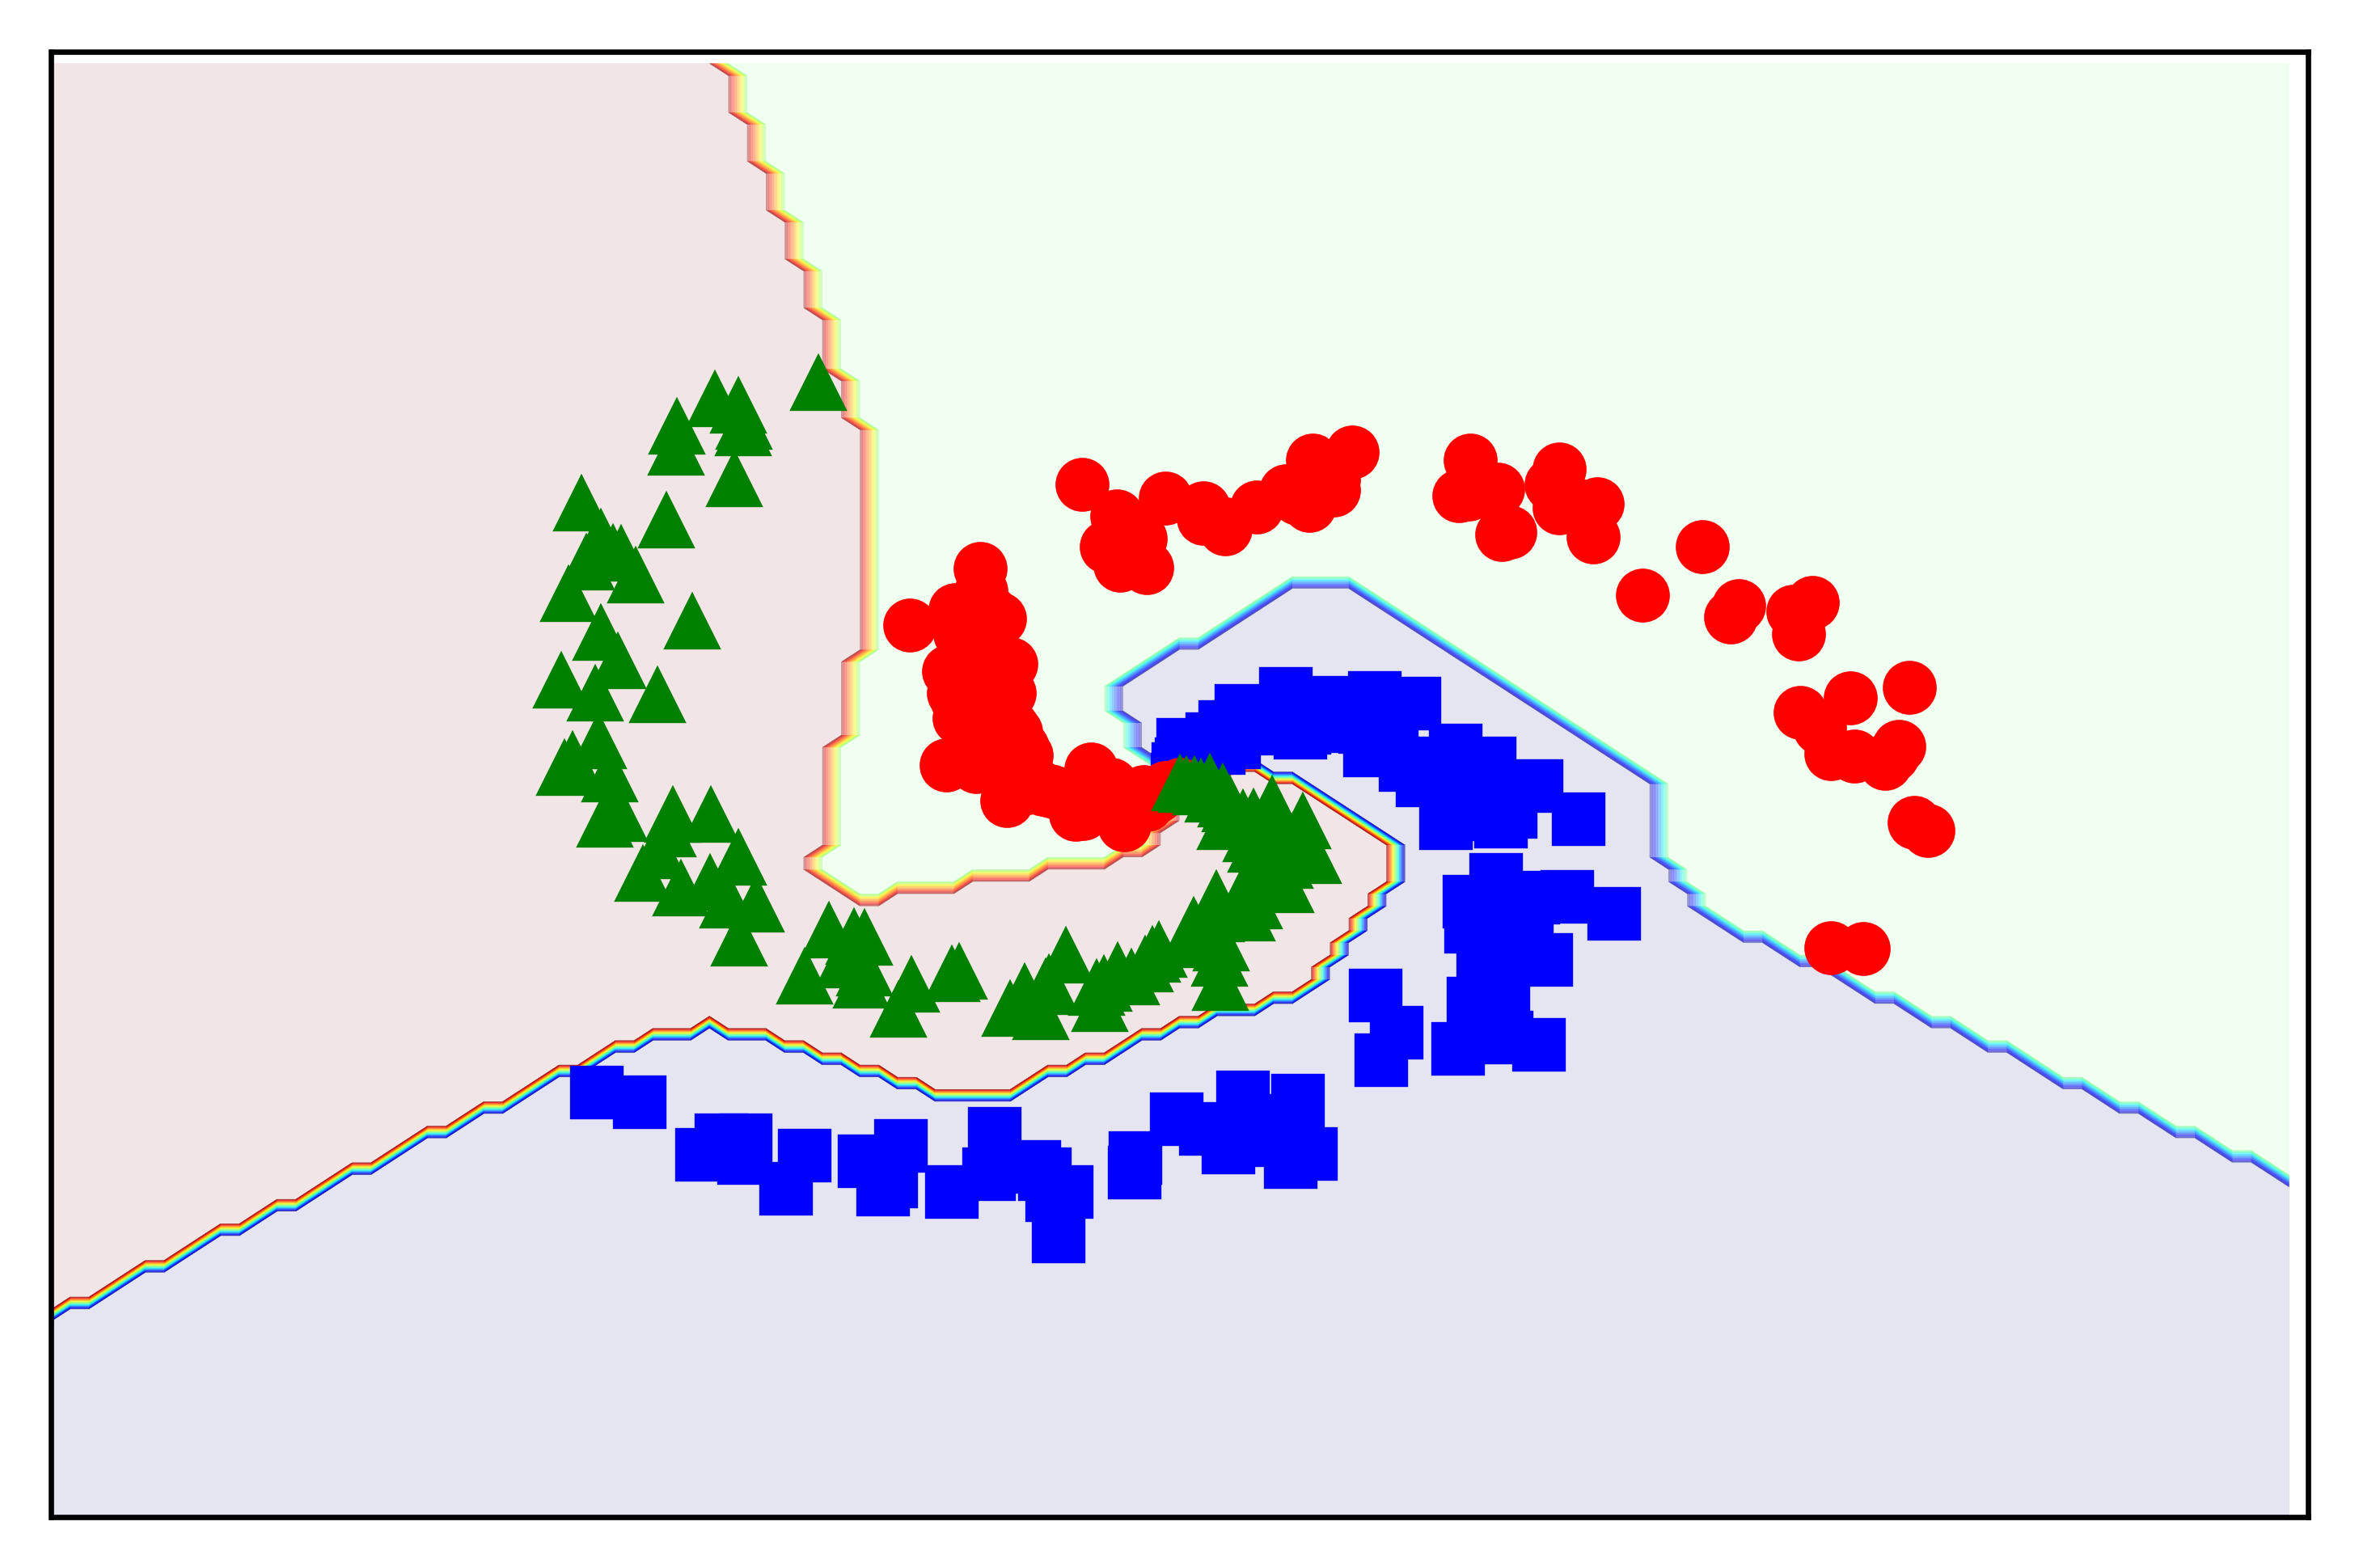
\includegraphics[width=1\linewidth]{EX500.png}
  \caption{K = 500}
  \label{fig:sub4}
\end{subfigure}
\label{fig:test}
\end{figure}

\end{document}

